% Two-pager research proposal: geometry-native neural midcurve extraction
% Intended as a back-to-back single sheet, for printing and circulation to
% prospective MS / PhD students.
% Build:  texify --engine=xetex -cp Main_TwoPager_MidcurveNN_GeometryResearch.tex
% (pdflatex also works; there is no Devanagari in this document.)

\documentclass[10pt,twocolumn]{article}

\usepackage[a4paper,margin=0.62in,columnsep=0.26in]{geometry}
\usepackage[utf8]{inputenc}
\usepackage[T1]{fontenc}
\usepackage{graphicx}
\usepackage{amsmath}
\usepackage{amssymb}
\usepackage{enumitem}
\usepackage{titlesec}
\usepackage[font=small,skip=3pt]{caption}
\usepackage{xcolor}
\usepackage[colorlinks=true,allcolors=blue!55!black]{hyperref}
\usepackage{microtype}

\graphicspath{{images/}}

% Tighten the layout so the whole brief lands on exactly two pages.
\titlespacing*{\section}{0pt}{6pt plus 1pt minus 1pt}{3pt}
\titlespacing*{\subsection}{0pt}{4pt plus 1pt minus 1pt}{2pt}
\titleformat{\section}{\normalfont\large\bfseries}{\thesection.}{0.5em}{}
\titleformat{\subsection}{\normalfont\normalsize\bfseries}{}{0em}{}
\setlist[itemize]{leftmargin=1.1em,topsep=2pt,itemsep=1pt,parsep=0pt}
\setlength{\parskip}{2pt}
\pagestyle{empty}

\newcommand{\shape}[1]{\textsf{#1}}

\begin{document}

\twocolumn[
\begin{@twocolumnfalse}
\begin{center}
{\LARGE\bfseries Learning the Medial Axis\par}
\vspace{3pt}
{\large Geometry-Native Neural Networks for Midcurve Extraction\par}
\vspace{5pt}
{\normalsize A research topic proposal for MS / PhD students\par}
\vspace{4pt}
{\small Yogesh H. Kulkarni \quad$\cdot$\quad
\href{https://github.com/yogeshhk/MidcurveNN}{github.com/yogeshhk/MidcurveNN} \quad$\cdot$\quad
\href{https://www.linkedin.com/in/yogeshkulkarni}{linkedin.com/in/yogeshkulkarni}\par}
\vspace{8pt}
\end{center}
\end{@twocolumnfalse}
]

\section{The problem}

Computer-Aided Engineering routinely replaces a thin three-dimensional solid
with a lower-dimensional idealization before meshing: a thin-walled housing
becomes a surface model, a slender bracket becomes a wireframe. Done well, this
cuts simulation cost by an order of magnitude while preserving the physics of
interest. Done badly, it silently corrupts the analysis.

The two-dimensional version is the \emph{midcurve} problem, and it is the
honest test bed for the general case: given a closed profile, produce the
polyline running down its middle --- its medial axis, cleaned of the spurious
branches classical algorithms generate at every convex corner.

Those classical transforms are exact but brittle: sensitive to boundary
perturbation, and dependent on pruning heuristics hand-tuned per shape family.
In production CAD, midsurfacing remains substantially manual. That is the gap a
learned method should close.

\begin{figure}[t]
\centering
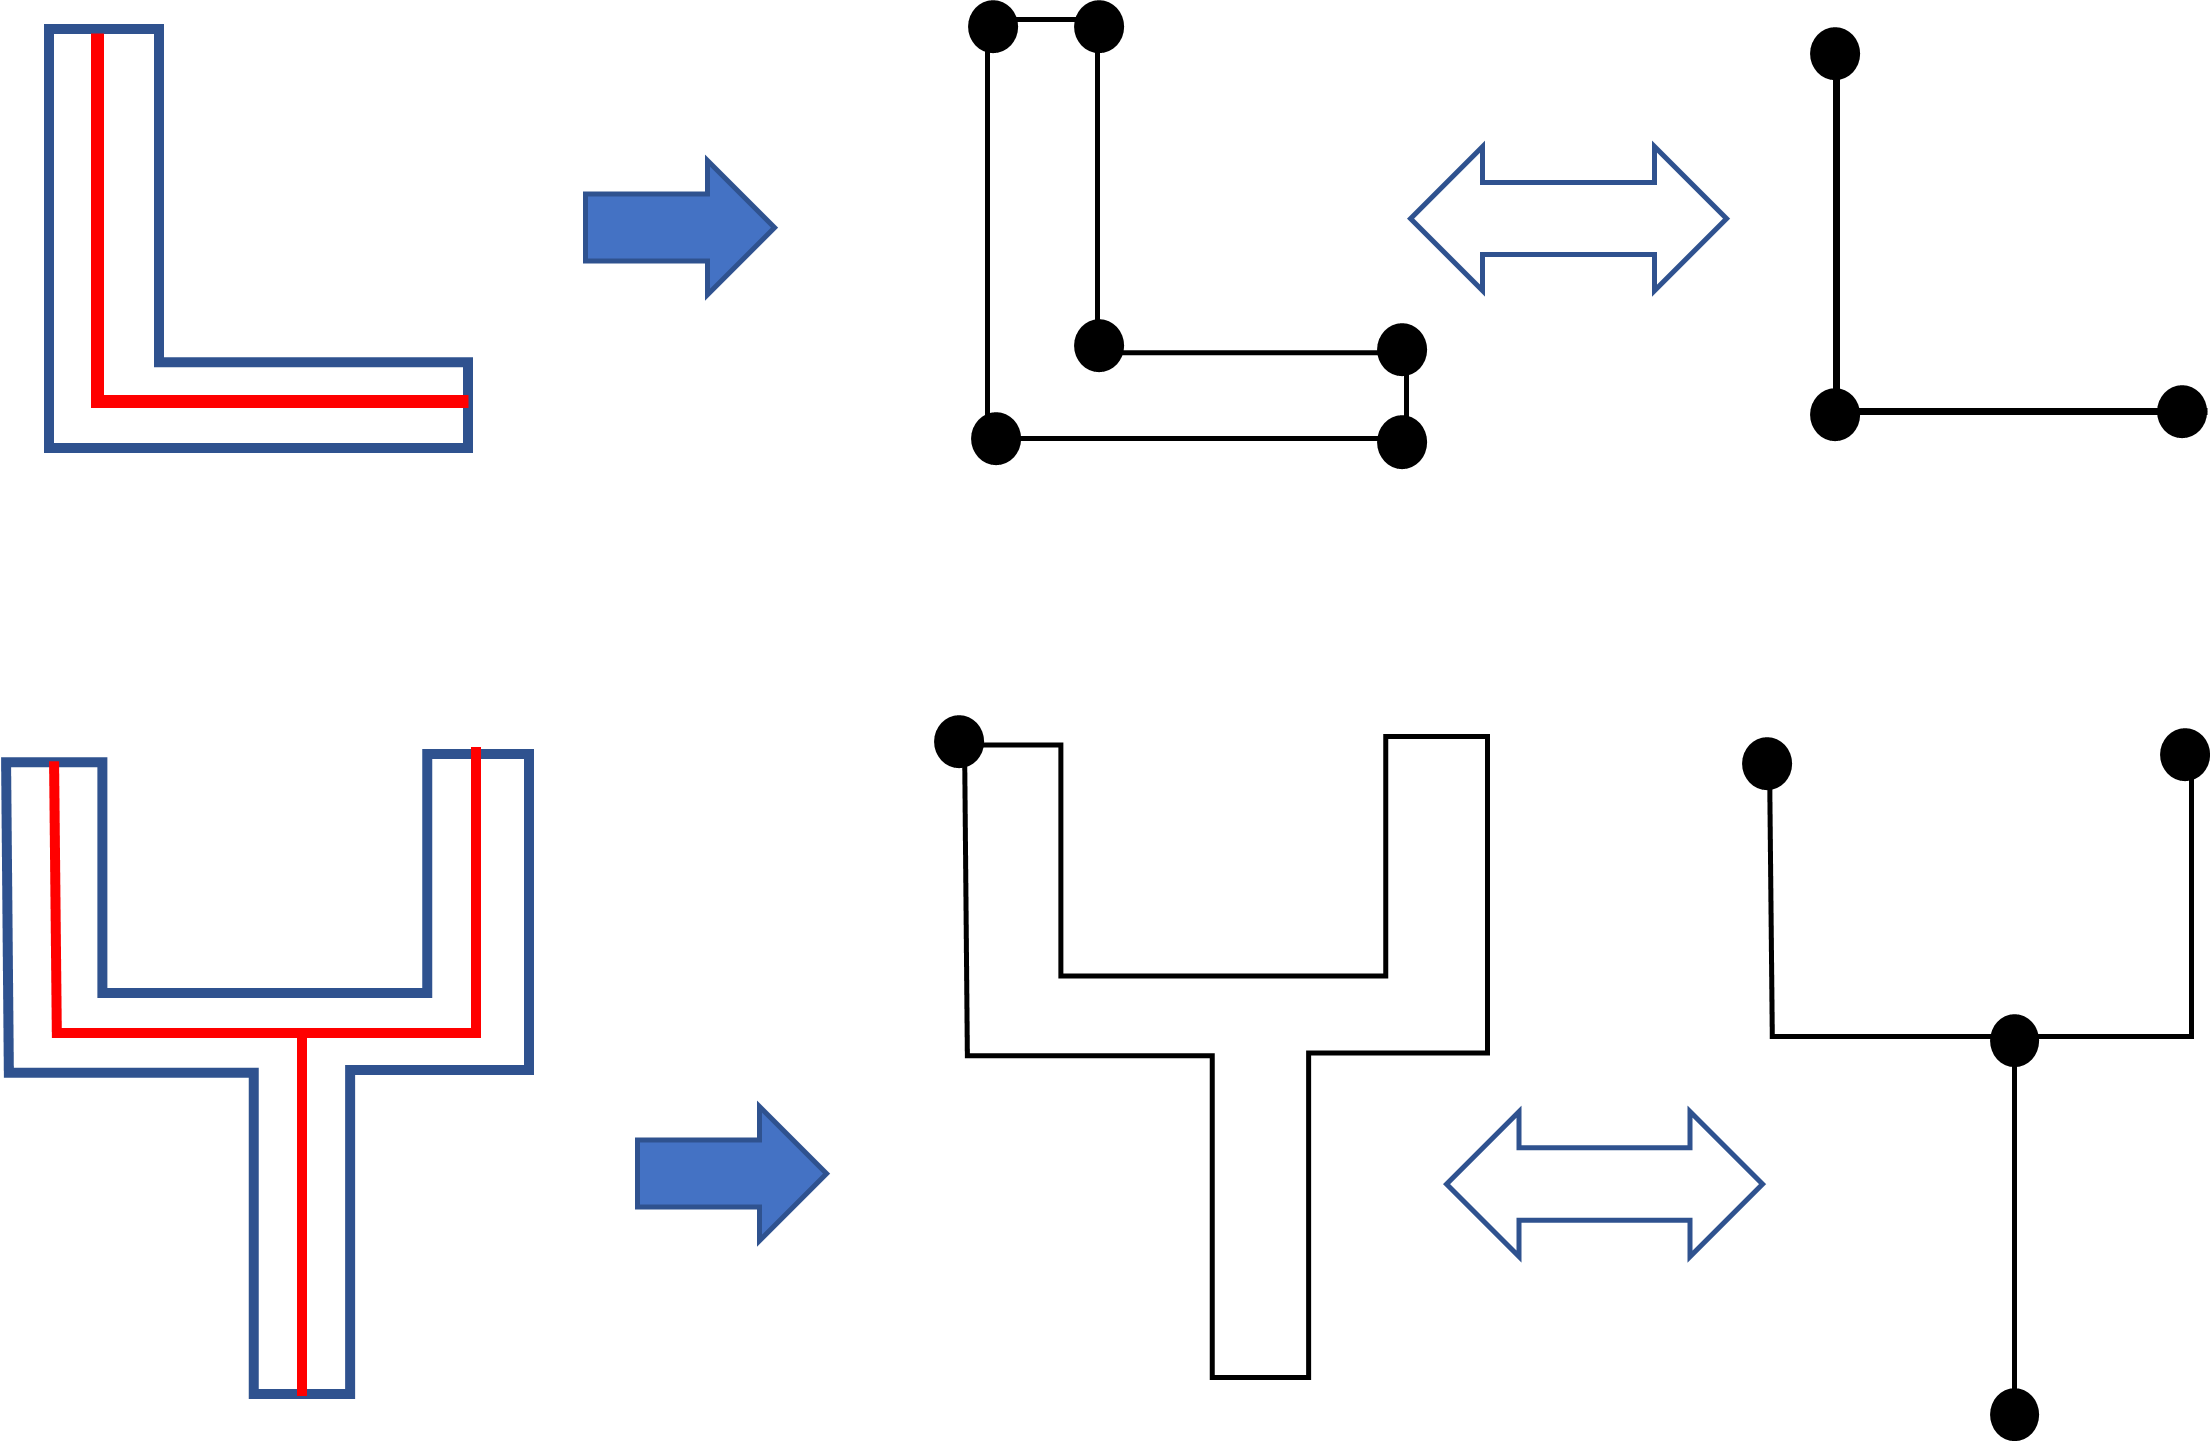
\includegraphics[width=0.86\linewidth,keepaspectratio]{midcurve_as_graph}
\caption{The transformation to be learned, stated natively. A closed profile
polygon (nodes = corners, edges = walls) maps to an open, possibly branched
midcurve graph. Node count, topology and manifoldness all change --- and almost
no standard graph-learning machinery assumes they can.}
\label{fig:asgraph}
\end{figure}

\section{What has been tried, and where it stops}

The \textsc{MidcurveNN} project has taken this problem through two complete
approaches. Both work, and both plateau for the same underlying reason.

\textbf{Phase I --- raster.} Rasterize the profile, learn a bitmap-to-bitmap
map with an encoder--decoder (a UNet variant is strongest of seven
implemented). It trains readily and produces recognizable midcurves --- but the
output is pixels. Recovering a clean polyline from a fuzzy raster is a second,
unsolved problem, and everything an engineer needs (exact coordinates,
connectivity, branch points) was discarded at the input stage.

\textbf{Phase II --- text.} Serialize the profile as boundary-representation
JSON and fine-tune a code LLM to emit the midcurve as JSON. This is the best
current performer and, unlike Phase I, emits exact coordinates and explicit
topology. Its limits are equally clear: it learns a serialization convention
rather than a geometric operation, offers no invariance guarantees under
rotation or scaling, and needs a 7B-parameter model for a problem whose
intrinsic dimension is tiny.

Both phases route a fundamentally geometric operation through a representation
that is not geometric. That is the observation this proposal starts from.

\section{The proposal: predict geometry as geometry}

Represent the profile as a graph --- nodes are polygon corners carrying
$(x, y)$, edges are walls carrying length --- and predict the midcurve as
another graph, directly in coordinate space (Figure~\ref{fig:asgraph}). Exact
coordinates in, exact coordinates out. Branching is native. Invariances can be
built into the architecture instead of being hoped for from data augmentation.

A first implementation exists in the repository: a non-autoregressive graph
transformer, plus a variant fine-tuned from a pretrained Graphormer backbone.
Its measured behaviour is the reason this is a research topic and not an
engineering ticket. Node positions are approximately learned, but the
adjacency cross-entropy sits at roughly $1.15$ --- indistinguishable from
chance. \textbf{The model learns where the midcurve points are and fails
entirely to learn how they connect} (Figure~\ref{fig:results}).

That failure is not a tuning problem. It follows from four open questions.

\section{The open research questions}

\subsection{Q1. Output sets of unknown size, without correspondence}

A profile with $N_p$ corners does not induce any fixed number of midcurve
nodes, and nothing tells the loss function which predicted node should
correspond to which ground-truth node. Chamfer distance sidesteps the question
and, in doing so, provides no usable gradient for topology: it can score well
while the connectivity is arbitrary.

The promising direction is set prediction in the DETR sense: a fixed pool of
learned queries cross-attending to the encoder, each emitting coordinates and
an existence probability, matched to ground truth by Hungarian assignment, with
adjacency supervised only on matched slots. Whether that recipe transfers from
object detection to exact geometry --- where coordinate error means a failed
part, not a loose bounding box --- is genuinely open.

\subsection{Q2. Topology as a first-class prediction target}

Predicting a $k \times k$ adjacency matrix with independent Bernoulli entries
does not encode what a midcurve is. A midcurve is connected, essentially
acyclic, and its branch points carry engineering meaning. A model that emits a
disconnected point cloud with a plausible-looking adjacency matrix has produced
nothing usable.

This calls for losses and decoders that are aware of graph structure ---
degree-consistency terms, spanning-structure extraction, differentiable
connectivity surrogates --- and for evaluation by edge F1 and branch-point
detection rate rather than by cross-entropy.

\subsection{Q3. Long-range geometric reasoning}

A midcurve point is, by construction, equidistant from two \emph{opposing}
walls. On a ring graph those two walls are maximally far apart in graph
distance. Three rounds of neighbourhood message passing cannot connect them:
the architecture is structurally incapable of forming the pairs that define the
answer.

Candidate remedies --- virtual global nodes, dense attention with random-walk
positional encodings, geometric node features such as interior angle and
arc-length position --- are individually well-understood. Which combination
suffices for medial-axis reasoning, and how it scales with polygon complexity,
is not.

\subsection{Q4. Generalization from a handful of topologies}

The public dataset has four base shapes: \shape{I}, \shape{L}, \shape{T},
\shape{Plus}. Every training row is a rigid or scale transform of one of them.
Any reported accuracy therefore measures interpolation, not generalization ---
a caveat that applies to all three phases and is documented as such in the
repository.

Honest progress needs leave-one-shape-out evaluation, a synthetic generator
producing rectilinear polygons with analytically known medial axes, and
augmentations that survive coordinate normalization (edge subdivision, in
particular, so the model cannot memorize node count as a proxy for shape).

\begin{figure}[t]
\centering
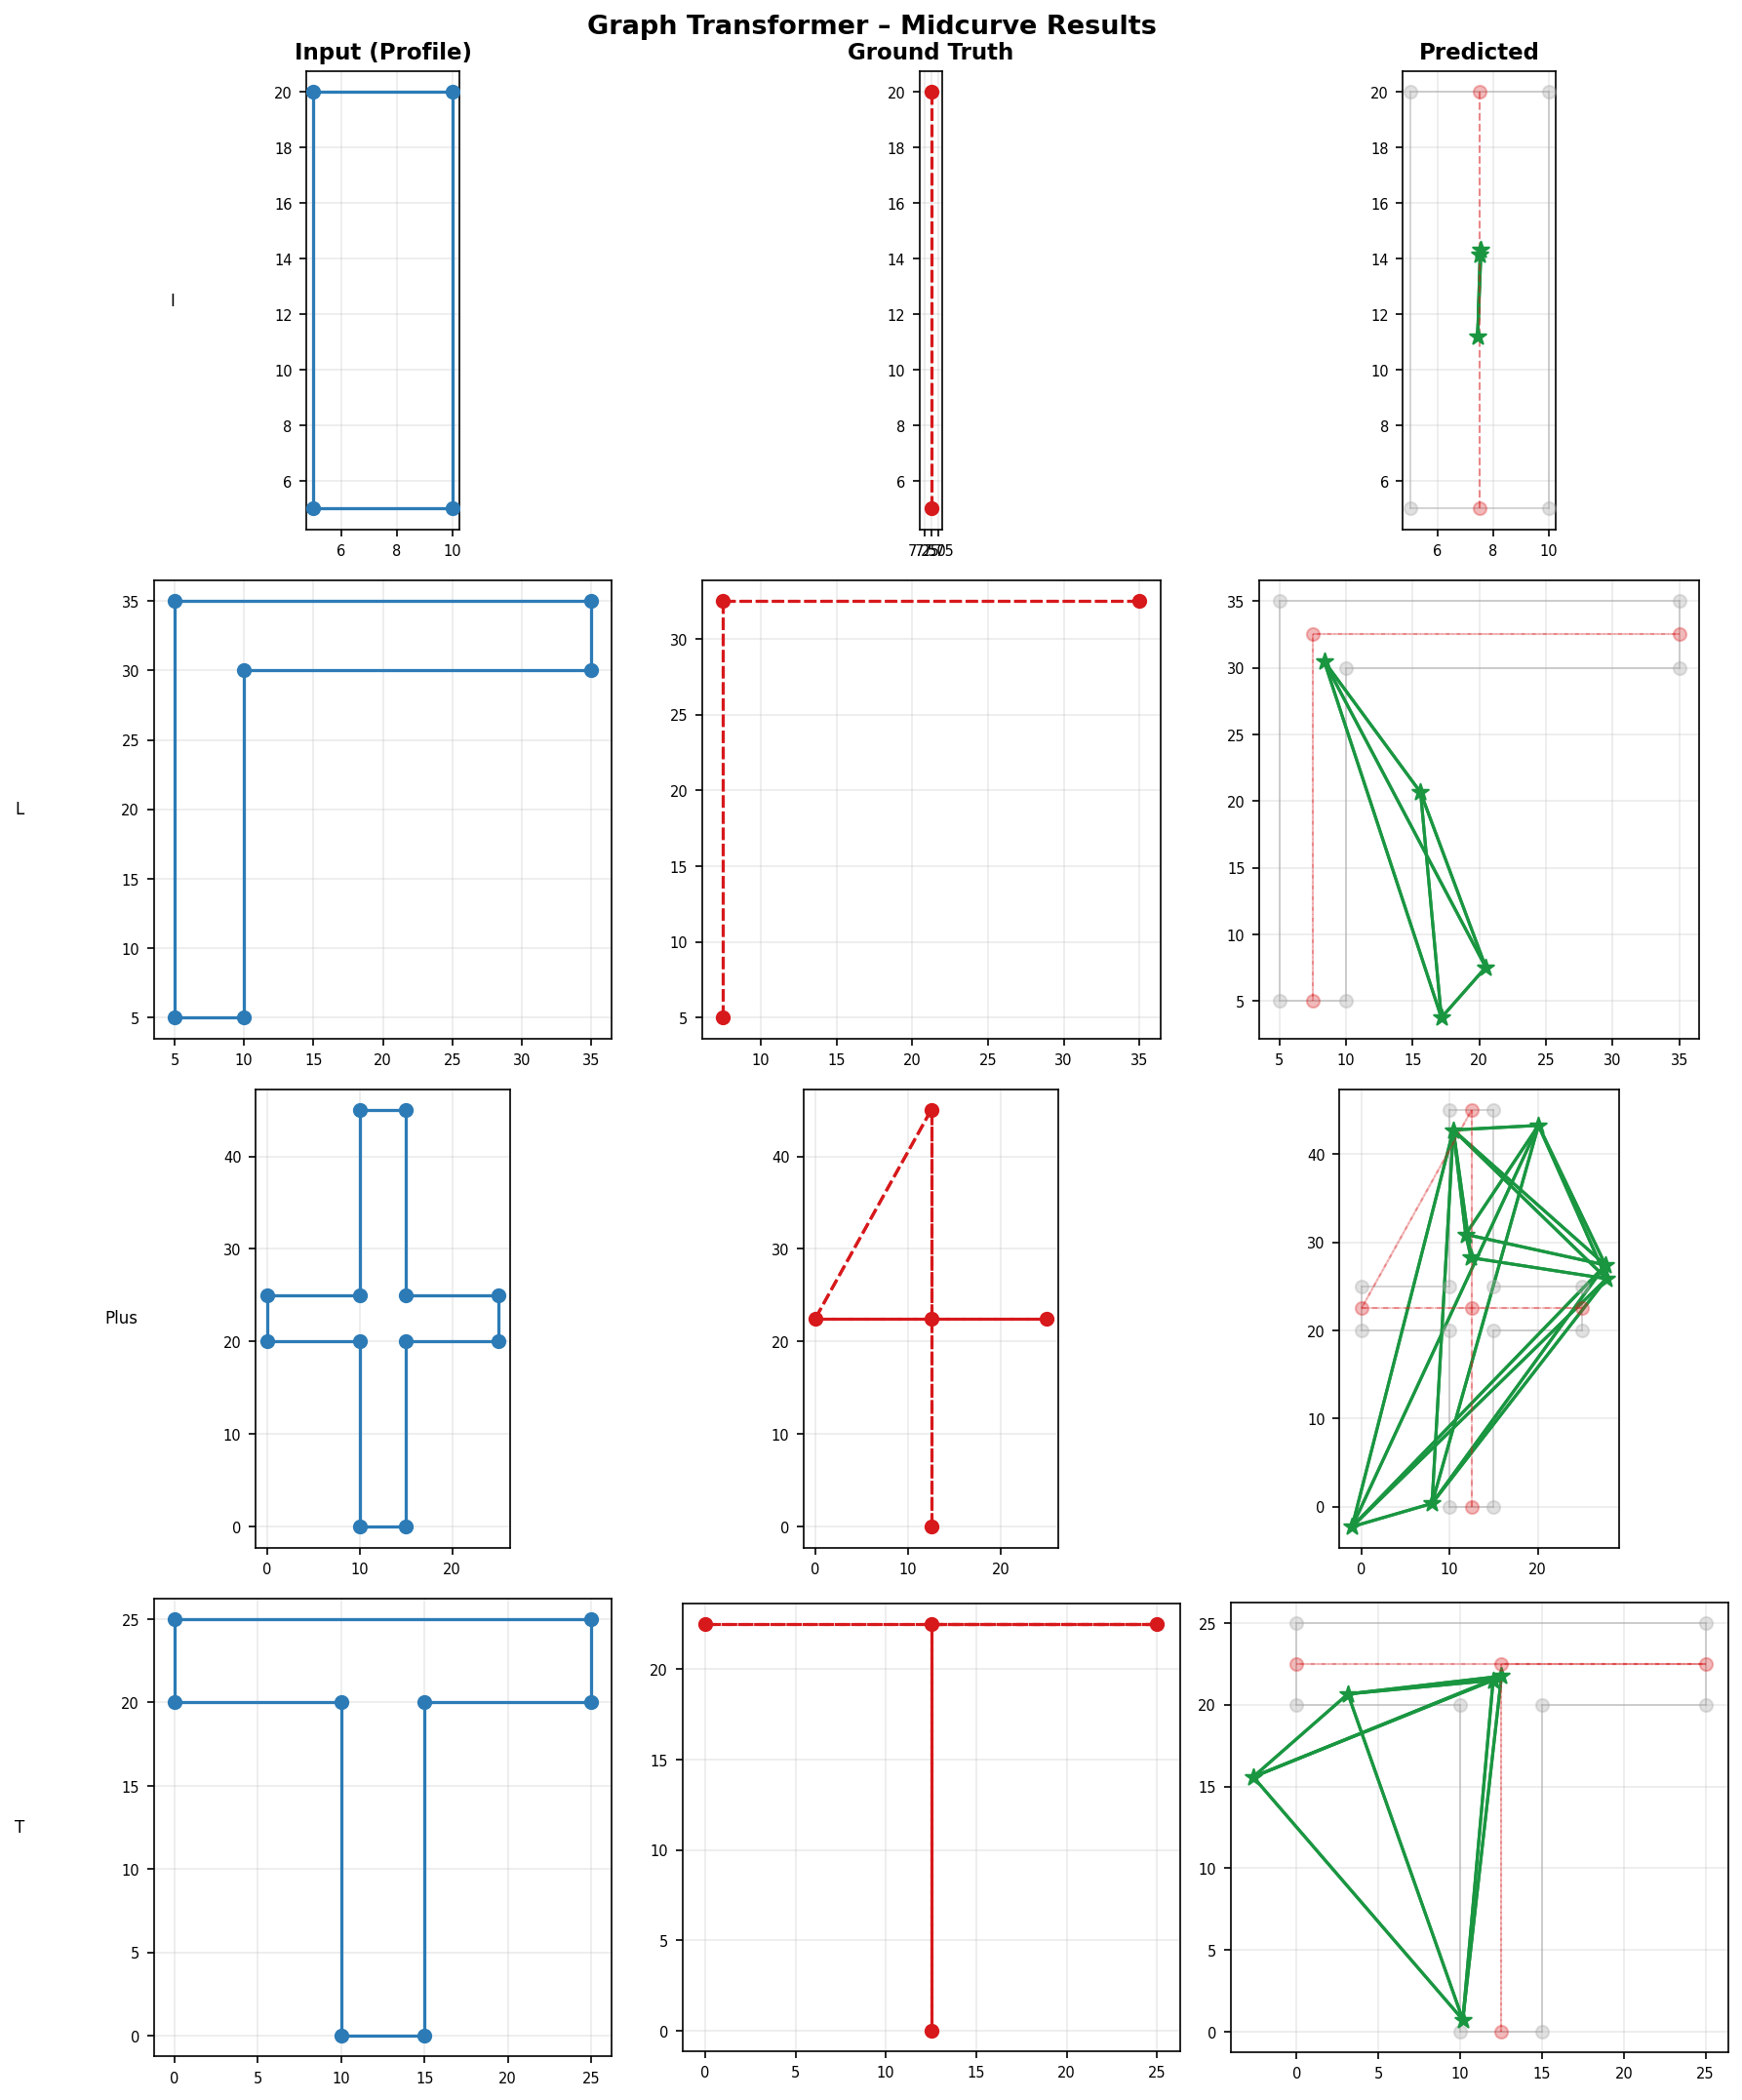
\includegraphics[width=0.86\linewidth,keepaspectratio]{graph_transformer_results_grid}
\caption{Current geometry-native baseline. Left to right: input profile,
ground-truth midcurve, prediction. Point placement is broadly plausible;
connectivity is not learned. Closing this gap is the core of the proposed
work.}
\label{fig:results}
\end{figure}

\section{Scope}

The questions decompose cleanly into two levels of commitment.

\textbf{Master's scope (one year).} Take Q1 and Q4. Implement the
set-prediction decoder with Hungarian matching, replacing the current pooling
decoder; build the synthetic data generator and the leave-one-shape-out
protocol; report edge F1, Hausdorff and branch-point metrics against the
existing raster and text baselines. Deliverable: the first honest
generalization number for this problem, and a decoder that handles variable
output size by construction.

\textbf{Doctoral scope (three to four years).} All four questions, plus the
generalization that motivates the exercise: \emph{closed to open} and
\emph{manifold to non-manifold} transformations, and the extension from
midcurve to midsurface. A thin solid does not reduce to one clean sheet, but to
a set of sheets meeting along non-manifold junctions. Learning maps whose
output topology differs structurally from their input topology, with guarantees
strong enough for engineering use, is a thesis-sized question reaching well
beyond CAD.

\section{What a student gets}

An unusually well-prepared starting point: three implemented approaches to
compare against, a benchmark harness, a documented catalogue of known failure
modes with file-and-line references, and prior publications to build on. The
problem is small enough to iterate on a single GPU and real enough that a
working solution has direct industrial use. It also sits in an active research
neighbourhood --- geometric deep learning, set prediction, neural methods for
CAD --- while staying concrete and evaluable.

\textbf{Prerequisites.} Python and PyTorch; some graph neural network exposure
(PyTorch Geometric); enough computational geometry to reason about medial axes.
CAD experience welcome, not required --- the geometry is elementary; the
learning problem is not.

\section{Getting started}

Code, data, analysis reports and prior publications are public at
\href{https://github.com/yogeshhk/MidcurveNN}{\texttt{github.com/yogeshhk/MidcurveNN}}
--- all three phases plus the benchmark harness. The specific starting point
for this proposal is \texttt{src/geometry\_based/analysis\_report.md}: fifteen
catalogued issues and nine prioritized research directions, each mapped to file
and line. Interested students, or supervisors looking for a co-supervised
topic, are welcome to open a GitHub issue or make contact via LinkedIn.

\vspace{4pt}
\hrule
\vspace{3pt}
{\footnotesize\noindent
\textbf{Selected background.}
Blum, \emph{A transformation for extracting new descriptors of shape} (1967)
--- the medial axis.\;
Carion et al., \emph{End-to-End Object Detection with Transformers} (ECCV 2020)
--- the set-prediction recipe behind Q1.\;
Kulkarni, \emph{Computing a well-connected midsurface} (PhD thesis, CoEP) ---
the classical treatment this work aims to replace.\par}

\end{document}
